\documentclass[11pt, oneside]{article} 

\usepackage[margin=1in]{geometry}
\geometry{letterpaper}

\usepackage[parfill]{parskip}
\setcounter{tocdepth}{4}

\usepackage{graphicx}
\graphicspath{ {./figures/} }

\usepackage{amssymb}
\usepackage{amsmath}

\usepackage{cite}

\usepackage{float}
\usepackage[labelfont=bf,textfont=md]{caption}

\usepackage{booktabs}

\title{Drugs with Sex-Linked Risk of ADRs}
\author{Payal Chandak}
\date{}

\begin{document}
\maketitle
%\tableofcontents

\newpage

\section{Introduction}

Adverse drugs reactions (ADR) are injuries or unwanted effects that occur as byproducts of drug use. In 2016, the cost of drug-related morbidity and mortality was estimated at \$528.4 billion, or 16\% of total healthcare expenditure for the year \cite{watanabe_cost_2018}. Studies have shown that approximately half of all ADRs are preventable \cite{hakkarainen_percentage_2012}. A patient identified with increased risk of ADRs can be prophylactically managed by adjusting drug dosage, increasing surveillance for ADRs and individualized education \cite{tharpe_adverse_2011}. 

Previous studies have clearly established that females bear a much greater risk of developing ADRs compared to males \cite{rademaker_women_2001,anderson_sex_2005,whitley_sex-based_2009,ofotokun_sex_2003,bigos_sex_2009,rodenburg_sex_2012,yu_systematic_2016,tharpe_adverse_2011,tran_gender_1998,drici_is_2001,stabile_gender_2014,colombo_gender_2016,makkar_female_1993} In particular, nervous system drugs (especially antidepressants), cardiovascular system drugs (especially antiarrythmics) and antiinfectives are widely established as posing an increased risk of ADRs to women \cite{tran_gender_1998,drici_is_2001, rodenburg_sex_2012, tharpe_adverse_2011, ofotokun_sex_2003,whitley_sex-based_2009}. The sex bias in antiinfective action is remarkably evident in antivirals for Human Immunodeficieny Virus (HIV), which at the time of drug development was mostly prevalent in men. As a result of male dominant patient populations in clinical trials, HIV antivirals now cause considerably worse ADRs in women \cite{ofotokun_sex_2003,whitley_sex-based_2009}.

Although sex-linkage in ADR risks has been deeply researched for some drug classes, a comprehensive understanding of sex-risks posed by individual drugs remains unavailable. Clinical studies are restricted to investigating only a few, specific drugs due to small sample sizes. Meta-analyses are too broad, using studies with varying drug information to generalize across wide drug classes. Neither approach is able to determine the composite sex-risk of a given drug across all its ADRs. A large scale understanding of sex risks of individual drugs would make it possible to tailor prescriptions by patient sex. Avoiding drugs with high sex risks could potentially minimize ADRs, reducing unneccessary pain, discomfort and hospitalizations. Moreover, the current understanding of sex risks is binary: either the risk is present or absent. A quantified, graded risk score for drugs posing sex risks would allow similar drugs to be compared by risks, helping practitioners minimize ADRs by picking the lowest risk possible. 

Here, we take a population approach to identifying drugs that pose an increased risk of ADRs to either sex. We further derive composite risk scores for each drug with a sex risk.

\section{Methods}

We identified individual drug-ADR pairs with sex-linked disproportionalities. Risk to either sex was quantified by combining severity and frequency. The adverse events in each drug-ADR pair were assigned severity rankings. We quantified frequency of each pair using multiple. All pairwise frequency measures were normalized for sex-risks associated with adverse events. Ultimately, frequency and severity of drug-ADR pairs were condensed into composite sex-risks for drugs. We validated these risks for consistency and accuracy 

\subsection{Identifying Drugs}

We identified drugs with disproportionate sex risks of ADRs, we used a standardized, de-duplicated version of the US Food and Drug Administration Adverse Event Reporting System (AEOLUS) \cite{banda_curated_2016}. Records with missing or nonsensical sex information were removed. We isolated drug-ADR pairs with significantly elevated incidence of the adverse event for either sex (male or female). We conducted $\chi^2$ tests on the 264,023 drug-ADR pairs in AEOLUS. After adjusting for multiple testing with bonferroni correction, we retained 6155 drug-ADR pairs (p$<$0.05) as significant. Further we dropped ADRs that were sex-exclusive (pregnancy,  menopausal, prostate) or irrelevant (gunshot wound or homicide), retaining 5914 drug-ADR pairs. 

\subsection{Quantifying Risk Factors}

\paragraph{Determining Severity}

For a given drug, the risk of ADRs to any population is influenced by their severity. Gottlieb et al. used Internet-based crowdsourcing to rank adverse events by their degree of physiological or psychological harm \cite{gottlieb_ranking_2015}. Ranging from 0 to 1, the magnitude of the rank increased as the adverse events was percieved to be more severe. Ranked ADRs were mapped from MedDRA terminology to AEOLUS' SNOMED CT terminology using public mapping, largely automatically and partially manually \cite{boyce_bridging_2014}. See Supplementary Materials for ADR ranking and mapping. 

\paragraph{Determining Frequency}

For a given drug, the risk of ADRs is also influenced by their probability of occurrence. Since drug prescription data was unavailable, ADR incidence could not be compared to drug usage across sexes. Instead, for the sub-population consuming a given drug, the sex ratio of a target ADR was compared to that of any other ADR. A 2$\times$2 contingency table for each drug-ADR pair was created as follows: 

\hfill
\begin{center}
\begin{tabular}{ |c|cc| } 
	 \hline
	  & Target ADR Present & Target ADR Absent \\ 
	 \hline
	 Target Sex & a & b \\ 
	 Not Target Sex & c & d \\ 
	 \hline
\end{tabular}
\end{center}
\hfill

The target sex was the sex that experienced a higher incidence of the adverse event. For some subpopulation of AEOLUS on drug X, if some ADR Y was observed more often in Males (target sex) then: $a$ was number of Males that experienced Y; $b$ was Males that experienced any ADR except Y; $c$ was Females that experienced Y; $d$ was Females that experienced any ADR except Y. 

From this contingency table, various measures of frequency were calculated. The Reporting Odds Ratio (ROR) has been standardly used to quantify sex associations in population data \cite{yu_systematic_2016,rodenburg_sex_2012}. In most cases, this ratio of odds acceptably approximates the ratio of risks. However, as probabilities become large, small changes in probabilites create significant deviations between the two. In some cases, Relative Risk (RR) is considered to be a more conservative and accurate estimation of population risks \cite{sheldrick_math_2017, cummings_relative_2009}. Another frequency measure, Likelihood Ratios (LR) combines sensitivity and specificity to calculate risk probabilities detached from the prevalence of the ADR. Calcualted using Equation \ref{eq:frequency}, all three measures uniquely captured frequency associated risk of ADRs. 

\begin{equation} \label{eq:frequency}
	ROR = \frac{a/c}{b/d}\ \ \ ;\ \ \ LR =  \frac{a/(a+c)}{b/(b+d)}\ \ \ ;\ \ \ RR =  \frac{a/(a+b)}{c/(c+d)}
\end{equation}

%\begin{equation} \label{eq:frequency_alt}
	%ROR = \frac{a/c}{b/d}\ \ \ ;\ \ \ LR =  \frac{\frac{a}{a+c}}{\frac{b}{b+d}}\ \ \ ;\ \ \ RR =  \frac{\frac{a}{a+b}}{\frac{c}{c+d}}
%\end{equation}

\begin{equation} \label{eq:normalize}\
	normalized\ x = \frac{x\ - minimum(x)}{maximum(x) - minimum(x)}
\end{equation} 

During calculations, the sex with higher incidence of the ADR was selected as the target sex. As a result, the magnitude of the frequency measures (always $>$ 1) was directly related to the frequency-associated sex-risk of ADR. Using Equation \ref{eq:normalize}, the frequency measures were independently normalized from 0 to 1 to yield three more frequency measures: normalized Reporting Odds Ratio (RORn), normalized Likelihood Ratio (LRn) and normalized Relative Risk (RRn). Ultimately the frequency-associated sex risk was quantified by 6 factors: ROR, RORn, LR, LRn, RR and RRn. 

\paragraph{Adjusting for Sex Bias of Adverse Events}

Female patients generally have a 1.5- to 1.7-fold greater risk of developing  ADRs \cite{rademaker_women_2001,stabile_gender_2014}. So for any drug consuming subpopulation, the sexes faced different ADR risks that were independent of drug consumption. To isolate the sex-risk posed by a drug, we corrected the drug-ADR frequency factors by the sex-risk posed by the adverse event. We identified adverse events with significant sex associations using $\chi^2$ tests to compare the observed sex ratio of a target ADR to the expected sex ratio of all other ADRs in AEOLUS. For significantly sex-biased adverse events (Bonferroni p $<$ 0.05), all 6 frequency measures were computed with the universe as the AEOLUS population instead of a drug-specific subpopulation. The individual drug-ADR frequency factors were adjusted by their respective adverse event frequency factors to normalize the frequency sex-risk posed by the drug. 

See Supplementary Materials for data on 5914 drug-ADR pairs, including adjusted frequency measures, severity ranking and target sex.

\subsection{Deriving Composite Drug Risk Scores}

We condensed the frequency and severity of numerous drug-ADR pairs into composite sex-risks using linear combination. Individual sex-risks were calculated for each drug-ADR pair with Equation \ref{eq:individual risk}. With Equation \ref{eq:composite risk}, we combined individual risks into composite risk scores for 385 unique drugs. The composite risk score captured the increased risk of adverse events from taking a particular drug to either sex. The magnitude communicated the difference in risk posed to males and females. Since the logarithmic transformation made risks symmetric, negative values denoted female risks and positive values denoted male risks.

\begin{equation} \label{eq:individual risk}
	Individual\ Drug\textnormal{–}ADR\ Risk = Adjusted\ Frequency\ Measure\ \times Severity\ Rank
\end{equation}

\begin{equation} \label{eq:composite risk}
	Composite\ Drug\ Risk\ = \log \bigg( \frac{\sum Individual\ Male\ Risks}{\sum Individual\ Female\  Risks} \bigg) \\
\end{equation}

Figure \ref{fig:network} demonstrates that the composite risk score for a drug expresses the divergence in ADR risk to males and to females. Smaller composite female risks (e.g Bupropion and Citalopram)  are illustrated in the more balanced distribution of pink and blue nodes. In contrast, large, negative composite risks (e.g Sertaline and Duloxetine) are explained by their high female propensity (i.e. more female ADR nodes than male). In this manner, the composite risk score denoted a comparative value across sexes rather than an absolute risk to a particular sex. 

To eliminate statistical bias, six composite risk scores were derived from the six frequency measures for each of the 385 drugs. We established consistency across risk scores for a given drug by verifying that all scores proposed a risk to the same sex, that is, they were either all positive (male risk) or all negative (female risk). Data for 322 drugs with consistent risks is provided in Supplementary Materials. Additionally, although six independent composite risks were calculated for each drug, we averaged the risk by RRn and risk by LRn to get one mean risk. While the LRn focuses on sex-ratio differences, the RRn focuses on ADR-ratio differences. Since both values are normalized onto the same scale, this mean risk was used as a proxy for the various scores. 

\subsection{Validation}

We conducted permutation analysis to determine the statistical significance of the composite drug risks. For the 5914 drug-ADR pairs, frequency measure and severity rank values were shuffled and composite risks were recomputed. We compared consistency our risk scores to consistency at random (see Table 1). To further investigate the reliability of risks derived for a particular drug, we considered the average sample size of patients across drug-ADR pairs and the number of drug-ADR pairs that contributed to the composite risk score (see Figure \ref{fig:reliability}). Additionally, we conducted a manual search of scientific literature (independently of our results) to find drugs known to pose increased sex-risk of ADRs. Keywords such as `sex', `gender', `adverse reaction', `women', `men', and `drug response' were used to identify both clinical and population approach satudies. Finally, to assess patterns in risk posed by drugs with similar mechanisms of action (MOA), we examined distribution of sex risks by their Anatomical Therapeutic Chemical (ATC) Classification System (see Figures \ref{fig:atc1} and \ref{fig:atc3}).

\section{Results}

Of 1506 drugs in AEOLUS, 322 drugs (21.4\%) are found to have a sex-linked risk of ADRs. As per Table 1, only 52\% drugs had consistent risk scores at random in contrast with the 84\% consistent drugs in our results. The majority of these consistent drugs (70.2\%) pose increased risks to women, as was expected in literature. Furthermore, in Figure \ref{fig:atc1}, the prevalence of drugs with female risk across ATC 1 classes, especially in anti-infectives for systemic use, nervous system drugs and cardiovascular system drugs was in agreement with literature \cite{tran_gender_1998, drici_is_2001, rodenburg_sex_2012, tharpe_adverse_2011}.

From manual literature search, 12 drugs were identified as suitable for corroborating our results. We excluded many overly specific drug-ADR risks found in literature because they were unequal comparisons with our comprehensive drug risks. As seen in Table 2, all drugs were expected to have female risks according to literature. In our results, 10 drugs agreed with literature (posing female risks) while 2 drugs, Nevirapine and Sotalol, disagreed (posing male risks). More specifically, Digoxin, a cardiovascular drug widely known to cause increased mortality in women, had a female risk per our results \cite{whitley_sex-based_2009,tharpe_adverse_2011,rademaker_women_2001}. 

Antiinfectives to treat HIV are well recognized to have worse side effects in women \cite{ofotokun_sex_2003,whitley_sex-based_2009}. Our results were mostly consistent with literature, predicting Efavirenz, Lamivudine and Ritonavir to have strong female risks. On the whole, 27.3\% of Direct Acting Antivirals (see Figure \ref{fig:atc3}) posed a female risk. However, we predicted Nevirapine with a male risk although literature showed a female risk \cite{ofotokun_sex_2003,whitley_sex-based_2009}. 

While results were predominantly congruent with literature, some inconsistencies warranted further investigation. Figure \ref{fig:reliability}A showed that both conflicting drugs had sample size less than 100 and ADR count less than 5. On the other hand, drugs agreeing with literature were evenly distributed across larger sample sizes and ADR counts. Thus, we concluded that drug risks derived from ADR count greater than 5 or sample size greater than 100 were likely to be reliable. 

Figure \ref{fig:reliability}B shows drug reliability separated by sex and colored by risk magnitudes. The most reliable drugs posed medium-to-low female risks. In comparison to evenly distributed female risks, male risks appeared to be unreliably clustered with low sample size and low ADR count. Nevertheless, most male risk drugs had sample sizes and ADR counts well above 100 and 5 respectively, and seemed reliable.

Drugs were grouped by ATC classes in Figures \ref{fig:atc1} and \ref{fig:atc3}. Within the same ATC class, some drugs had female risks while others had male risks. For example, 29.4\% of all antidepressants posed an increased risk to women while another 11.8\% of antidepressants posed a risk to men. The figures demonstrated that drugs with similar MOAs posed varying risks to both sexes. 

\section{Discussion}

In accordance with scientific literature, sex risks found were predominantly female after ruling out confounding factors (disproportionate reporting in AEOLUS, sex bias of adverse events, bias in frequency calculations). 

The prevalence of female risks has been explained by sex differences in pharmacokinetics and pharmacodynamics \cite{rademaker_women_2001, tran_gender_1998,anderson_sex_2005, drici_is_2001}. Antidepressants, wherein the pharmacokinetics and drug-response time are known to substantially vary by sex, were accordingly found to have diverging sex risks (29.4\% Female, 11.8\% Male) \cite{bigos_sex_2009,rademaker_women_2001}. Drugs with lower hepatic clearance in women have female risk in our results: specficially Temazepam, Acetaminophen and Digoxin had the risks -1.35, -1.08, and -0.20 \cite{rademaker_women_2001,tharpe_adverse_2011}. 

Unlike men, women consume contraceptive, pregnancy and menopausal drugs concomitantly with other medication \cite{borda_studies_1967}. The potential risk of drug-drug interactions further explains the prevalence of female-risks in our findings. For instance, Acetaminophen was found to conjugate 50\% more in women on oral contraceptives compared to controls \cite{rademaker_women_2001}. Thus, many risks proposed in our results seem to have either clinical validation or a plausible physiological basis, warranting further investigation. 

However, women not only use more sex-specific drugs but they also take more medications simultaneously. In AEOLUS, women are consistently older than men. Both age and polypharmacy have been established as risk factors for ADRs and could be the underlying cause of female risks. {(32,33)}\cite{rademaker_women_2001} Not adjusting for these covariates is a significant but amendable limitation of our work. 

Of the 322 drugs proposed to have sex-linked risks, only 3\% have been clinically established to our knowledge. Most of the novel risk scores were dervied from large enough sample sizes and ADR counts (see Figure \ref{fig:reliability}) to be considered reliable. These novel findings provide an opportunity to tailor drug prescription by patient sex. Moreover, our method can be used to investigate ADR risks of other demographics such as age and ethnicity to further optimize treatment decisions.

Minimizing ADRs is a priority, especially when adverse events are severe. A physician at Columbia University Medical Center revealed that limited information available on single drug-ADR pair risks is primarily useful for specific concerns. Decision support resources like UpToDate lack broadly applicable prescription guidelines for sex risks of ADRs. Although ideally drugs with high sex risks should always be avoided, treatment benefits can outweigh the ADR risk of prescription \cite{paepe_drug_2013}. Nevertheless, if benefits of two drugs are acceptably similar, the physician agreed that knowledge of sex-risks of both drugs would motivate treatment decisions. Thus, access to global, interpretable sex risks would supplement and enable informed medical decision making, thereby minimizing ADRs.

In the past however, only a small proportion of computer-identified drug interactions have had clinically significant adverse reactions \cite{paepe_drug_2013}. Hence, the most clinically relevant sex-risks must be determined before using these risks in drug management. Drugs with the strongest clinical implications can be identified by harnessing Electronic Health Records to examine our population-based findings. Furthermore, some drugs proposed to have sex-risks could be false positives identified due to the selection and reporting bias in AEOLUS. \cite{banda_curated_2016} This limitation can be improved not only by adjusting for under- and over-reporting but also by conducting the same study on adverse event data from other independent populations and corroborating results. 

Drugs within ATC classes are often interchangeable and equivalent regarding treatment benefits because they have similar MOAs. This has prompted the assumption that drugs with similar MOAs pose similar ADR risks. Literature often generalized sex risks of entire drug classes based on the findings of a few drugs. \cite{bigos_sex_2009,drici_is_2001,ofotokun_sex_2003} However, our results surprisingly indicate that drugs within an ATC class pose different ADR risks to males and females. This novel suggestion should be pharmacologically investigated and clinically confirmed.  

\newpage
\section{Tables and Figures}
\bigskip

\textbf{Table 1: Permutation Analysis of All Drug Risks.}
\medskip\\
\begin{tabular}{lcccc}
\toprule
{} & All Consistent & 1/6 Conflicts & 2/6 Conflicts & 3/6 Conflicts \\
\midrule
Results & 85\% &   3\% &  11\% &  0.75\% \\
Random  & 52\% &  20\% &  19\% &  9\% \\
\bottomrule
\end{tabular}
\bigskip
\bigskip
\bigskip

\textbf{Table 2: Literature Validation of Individual Drug Risks.}
\medskip\\
\begin{tabular}{llcl}
\toprule
Drug Class & Drug Name &  Mean Risk Score & Risk in Literature \\
\midrule
Antiinfectives & Efavirenz & -1.04 &  Female \cite{whitley_sex-based_2009} \\
               & Lamivudine & -2.50 &  Female \cite{ofotokun_sex_2003} \\
               & Nevirapine &  1.08 &  Female \cite{ofotokun_sex_2003, whitley_sex-based_2009} \\
               & Ritonavir & -3.17 &  Female \cite{ofotokun_sex_2003} \\
\midrule
Cardiovascular System & Acetaminophen & -1.08 &  Female \cite{rademaker_women_2001, tharpe_adverse_2011} \\
               & Amiodarone & -4.88 &  Female \cite{drici_is_2001} \\
               & Digoxin & -0.20 &  Female \cite{whitley_sex-based_2009, rademaker_women_2001, tharpe_adverse_2011} \\
               & Metoprolol & -0.60 &  Female \cite{whitley_sex-based_2009} \\
               & Sotalol &  1.26 &  Female \cite{drici_is_2001} \\
\midrule
Nervous System & Citalopram & -0.88 &  Female \cite{tharpe_adverse_2011} \\
               & Fluoxetine & -1.30 &  Female \cite{bigos_sex_2009} \\
               & Sertraline & -1.48 &  Female \cite{bigos_sex_2009} \\
               & Temazepam & -1.35 &  Female \cite{rademaker_women_2001} \\
\bottomrule
\end{tabular}
\medskip\\
! indicates conflicting sex in results and literature. Negative risk score signifies female risk. Positive risk score signifies male risk.

\begin{figure}[H]
	\centering
	\makebox[\textwidth][c]{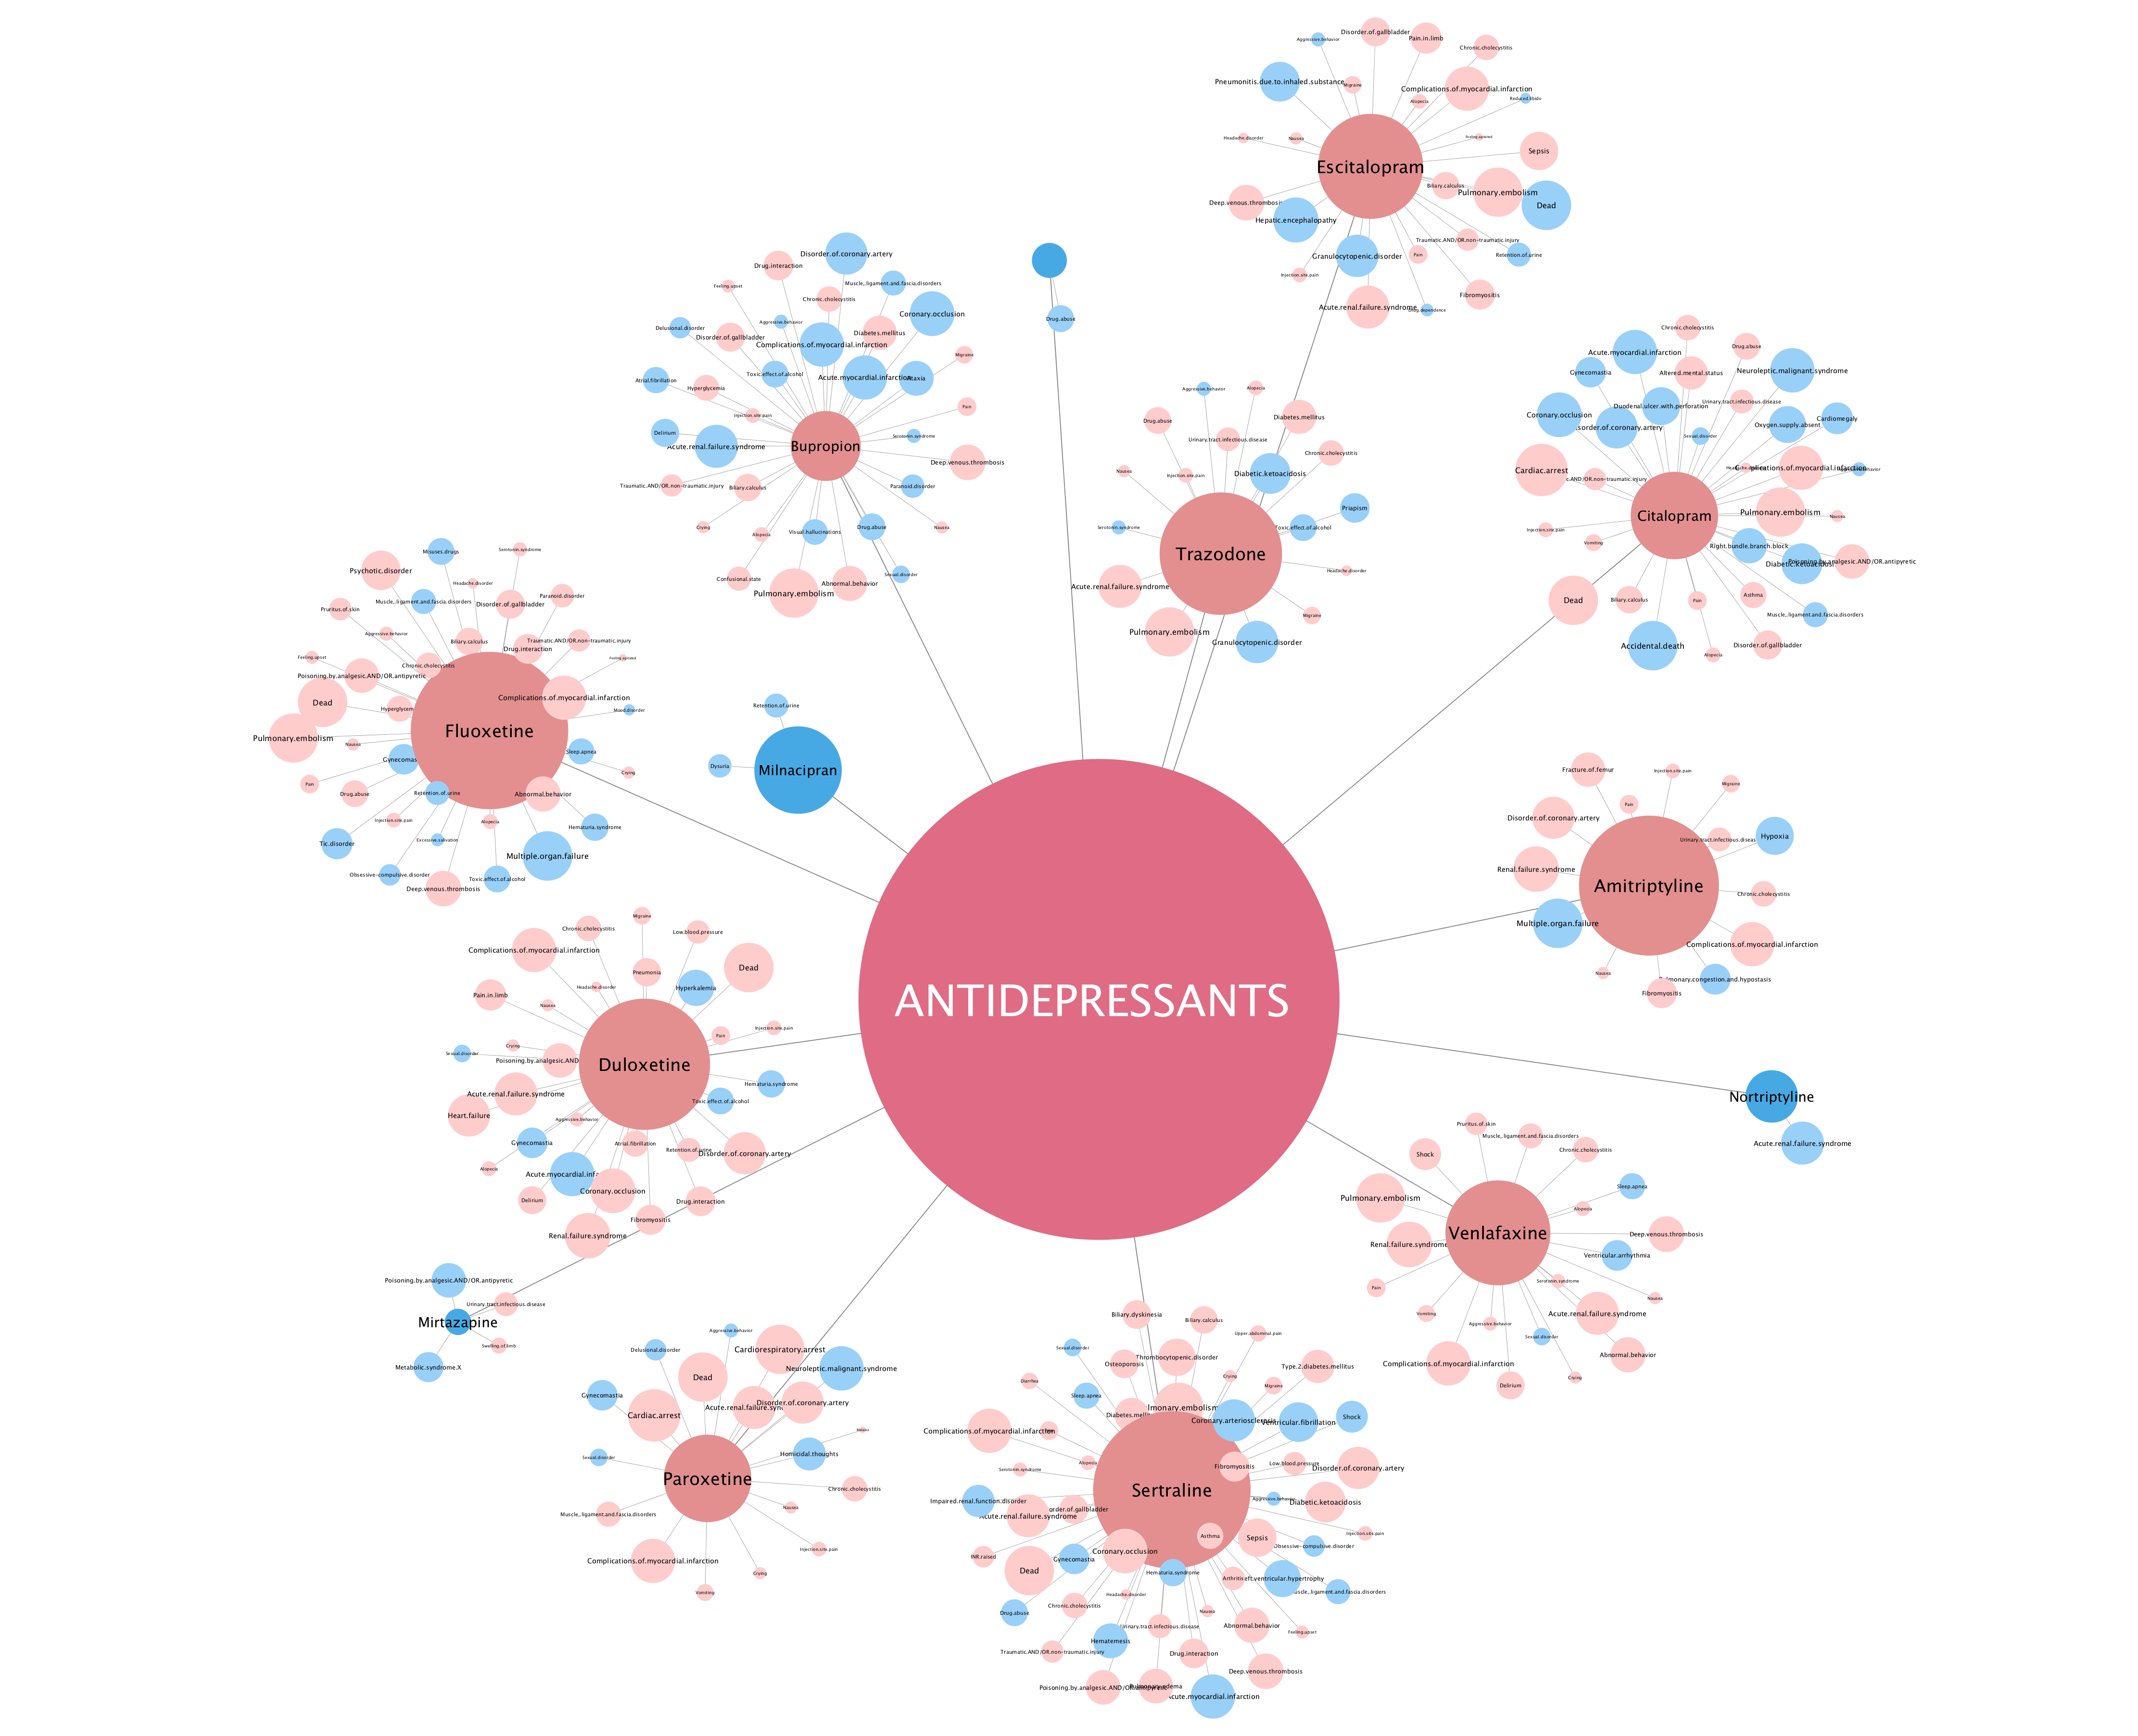
\includegraphics[width=1.4\textwidth]{antidepressants}}
	\caption{\textbf{Network Illustration of Drug Risks.} Antidepressant network illustration of individual drug-ADR risks converging into composite drug risks. Drug nodes are colored by sex at risk (pink for female, blue for male) and sized by composite risks. Drugs are linked to adverse events that contributed to their risk score derivation. Adverse Event nodes are colored by sex at risk and sized by severity rank.}
	\label{fig:network}
\end{figure}

\begin{figure}[H]
	\centering
	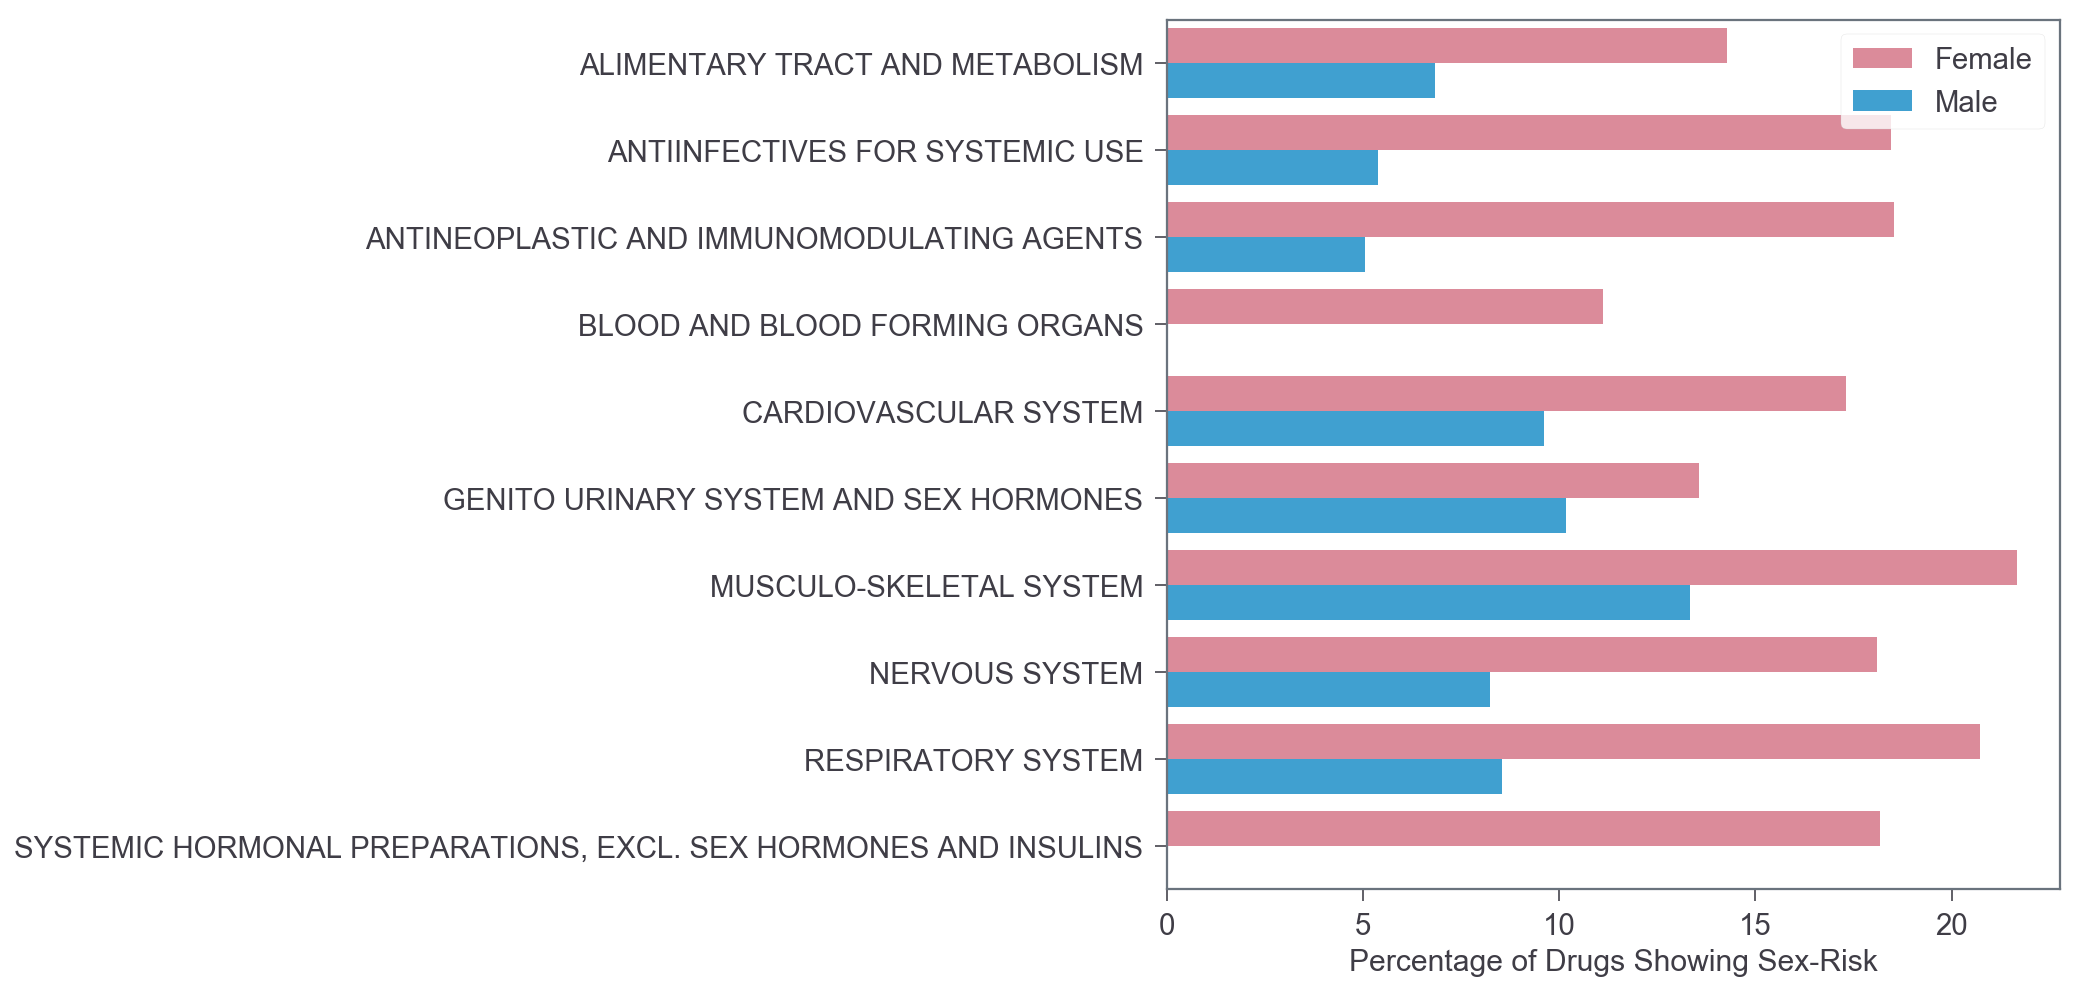
\includegraphics[width=\textwidth]{atc1}
	\caption{\textbf{Sex Risks in ATC 1 Classes.} Drugs posing ADR risk to either sex as a percentage of the total drugs in each ATC 1 class.}
	\label{fig:atc1}
\end{figure}

\hfill

\begin{figure}[H]
	\centering
	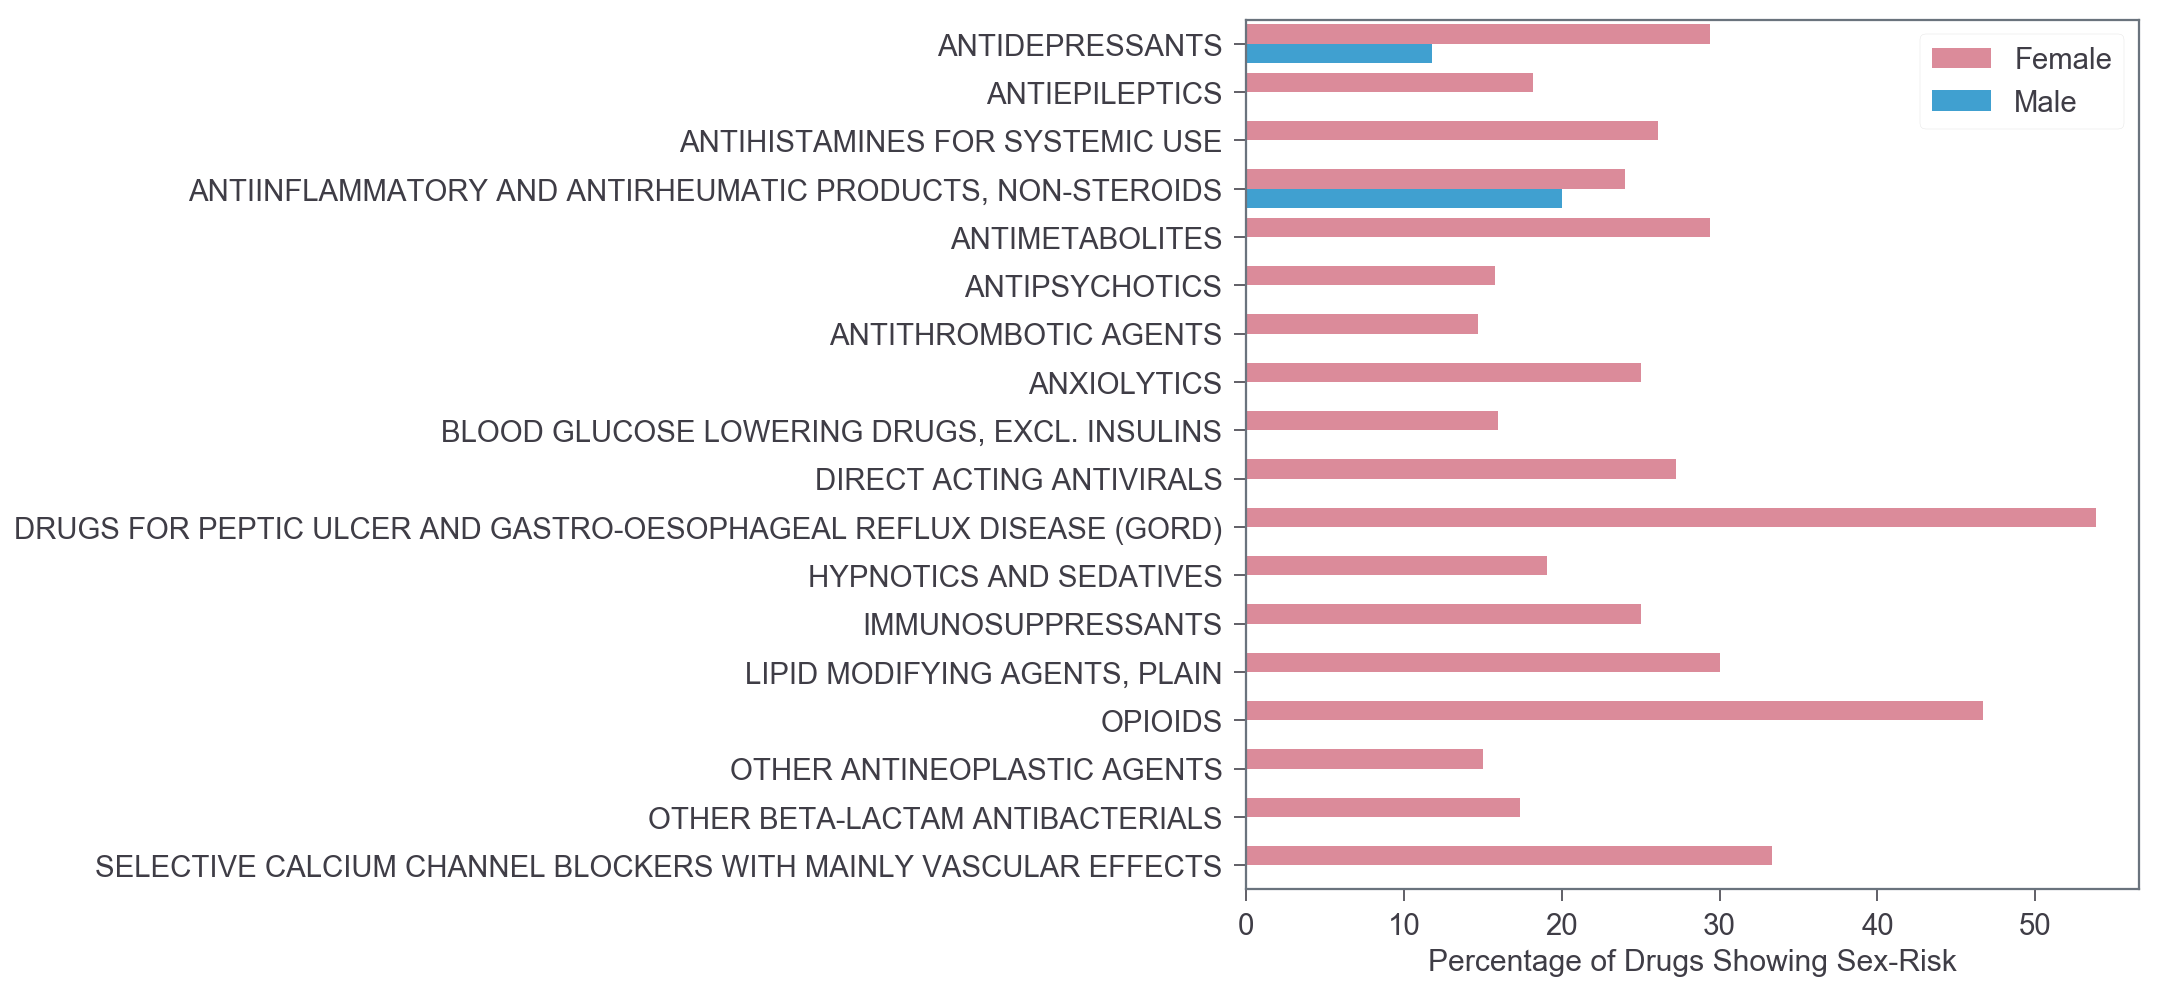
\includegraphics[width=\textwidth]{atc3}
	\caption{\textbf{Sex Risks in ATC 3 Classes.} Drugs posing ADR risk to either sex as a percentage of the total drugs in each ATC 3 class.}
	\label{fig:atc3}
\end{figure}

\begin{figure}[H]
	\centering
	\includegraphics[width=\textwidth]{reliability}
	\caption{\textbf{Reliability of Drug Risk Scores.} Drug risk distributed by number of adverse event outcomes and sample sizes used in deriving risks. \textbf{A.} Drugs validated in literature are highlighte for comparison against novel findings. \textbf{B.} Reliability distributions of all drugs separated by sex (red for female and blue for male) and colored by magnitude of risk score.}
	\label{fig:reliability}
\end{figure}

\newpage

\bibliographystyle{abbrv}
\bibliography{Bibliography}{}

\end{document}  

